\documentclass[./4_GeneralApproach.tex]{subfiles}
\graphicspath{{\subfix{../../Images}}}

\begin{document}
Fig. \ref{fig:contract_based_architecture} summarises the contract-based specification of the general system.

\begin{figure}[htp]
    \centering
    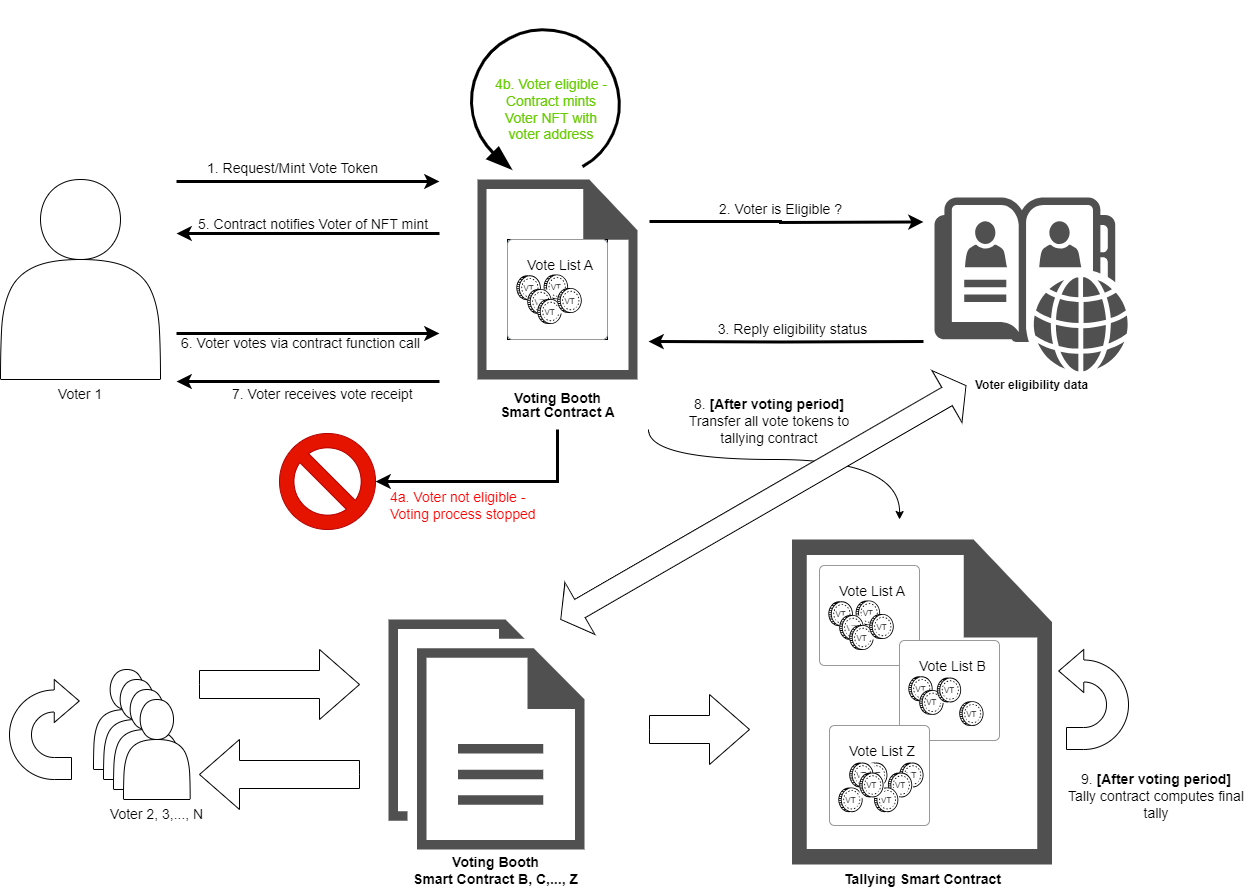
\includegraphics[width=0.7\textwidth]{../Images/02_contract_based_solution.png}
    \caption{Contract-based version of the e-voting system proposed.}
    \label{fig:contract_based_architecture}
\end{figure}

The crucial aspect to take into account with this version is how contract-based blockchains store smart contract-related data. All data related to a smart contract, from token ownership records to token metadata (in the case of NFT-generating smart contracts), is stored "into" the contract, i.e., in a block array referenced from the block where the contract was deployed. Ethereum, the best example of a contract-based blockchain, establishes the storage space for each contract as an "astronomically large array" starting from the deployment address of the smart contract, and extending it by $ 2^{256} $ slots of 32 bytes each, a number close to the number of atoms in the visible universe, hence the astronomical adjective. Ethereum simplifies storage under this model by skipping 0 (zero) values, i.e., only non-zero data is actually stored in the blockchain. For example, if a contract establishes a counter initialised to 0 as an internal parameter, as long as this variable retains the value 0, there is no blockchain storage used to store this value. Ethereum reserves a slot upon declaring the variable, but no write effort happens until that variable changes.
\par
Simple parameters are stored sequentially from the deployed address, using as many slots as required to fit all the required data. Arrays and mappings in Ethereum have a dynamic nature in the sense that they can be initialised as empty but can append and remove elements at will. This structures require a more complex storage system to allow for arbitrary grow, but they still get stored within the same "astronomically large" storage space.
\par
In this approach, all storage locations are identified by the base deployment address and the index of the slot where that particular data piece begins to be stored. The actual data can extend itself over several consecutive slots, an approach similar to how the data of a given file in modern operating systems is spread through several storage blocks (which in this case do not need to be arranged consecutively), which implies that if this base address is lost, so do the rest of the data stored using this reference point.
\par
In the system indicated in Fig. \ref{fig:contract_based_architecture} represents a system that uses this approach to save data. Voters start the process by interacting with the voting booth smart contract and request a Ballot NFT for a given election. Towards this, voters provide the required data to infer over their eligibility for the voting exercise at hand. If found viable, the contract mints a new Ballot NFT to the voter, which consists in creating a set of concurring entries in a set of internal mappings that uniquely establish the ownership of that Ballot NFT to a single voter.
\par
When the voter receives confirmation that he/she "owns" a Ballot NFT, it means that there a series of records in a voting booth smart contract editable by the voter and no one else. This is the essence of token ownership in a contract-based scenario. From here, the voter interacts again with the contract but now to change the token metadata according to his/her election choices. This change occurs in the smart contract data stored in the blockchain. The contract limits the edition of token metadata to its owner, but this data is stored under the contract's storage space, so voting in this scenario realistically changes the contract data stored in the blockchain.
\par
From here, the rest of the process consists in changing the ownership records in the contract to reflect the new ownership changes. After minting, the ownership of a Ballot NFT is transferred to the voter that requested it. After voting, the voter transfers the token back to the voting booth contract. From the blockchain standpoint, this consists in changing the owner address in the corresponding contract mapping from the voter account to the deployment address of the contract. This process can be repeated multiple times for a single voter if he/she decides to recast or revoke the last Ballot NFT submitted. Once the voting window closes, the voting booth contracts remove the data that links a stored Ballot NFT to a voter, a requirement to allow for recasting or revoking Ballot NFTs, and transfers the anonymised ballots to a tallying contract. This contract finishes the election process by removing the last layer of encryption, tallying, and publishing the election results
\end{document}